\section{Proyecto principal}
%
%
Este trabajo trataba de la optimización del gasto energético de una empresa que contaba con hornos de fundición. Para ello, se tuvieron que realizar predicciones del precio de la electricidad mediante modelos estadísticos. Posteriormente, se modelizó el proceso de fundición llevado a cabo en la fábrica y por último se trató de optimizar la selección de los materiales a fundir, dependiendo del espacio disponible en fábrica y el precio de la luz en cada tramo horario, estimado previamente.\\

A continuación, muestro una introducción a cada una de las partes mencionadas, con ejemplos o explicaciones del proceso. Como se ha dicho anteriormente, por motivos de confidencialidad no se pueden mostrar resultados o código explícito porque podría involucrar datos privados del proyecto o de la empresa cliente.
%
%
\subsection{Predicción de precios de la luz}
%
%
%
%
Para llevar a cabo la predicción del coste energético, se procedió en primer lugar al análisis de la serie temporal de precios de la electricidad. Este incluyó la generación de diversas gráficas, tales como series de tiempo o diagramas de autocorrelación simple (ACF) y parcial (PACF), con el fin de comprender la estacionalidad y el comportamiento de la varianza.\\

Concretamente, se utilizó como fuente de datos el mercado diario SPOT de electricidad en España. Los datos se obtuvieron a través de la API pública proporcionada por ESIOS (Sistema de Información del Operador del Sistema Eléctrico), que permite acceder a los precios horarios históricos, así como a otros indicadores del sistema eléctrico.
%
%
%
\subsubsection{Estudio y comprensión del mercado}
%
%
%
Antes de abordar la predicción, se realizó un estudio del funcionamiento del mercado eléctrico español y de la normativa que afecta a las industrias electrointensivas. Esta revisión fue clave para entender qué variables influyen realmente en la factura energética de un cliente industrial, más allá del precio medio horario.\\

Por ejemplo, el cliente indicó que una parte importante del coste final se debía a excesos en el consumo en ciertas franjas horarias o a penalizaciones asociadas a picos de demanda. Esto motivó no solo la necesidad de predecir el precio por hora, sino también de incorporar restricciones operativas en la fase de optimización basadas en el conocimiento regulatorio del sector.
%
%
%
\subsubsection{Obtención de los datos}
%
%
%
Los datos horarios del precio de la electricidad se descargaron mediante la API de ESIOS, para un rango histórico de 2023-2025 con el fin de capturar tanto patrones estacionales diarios como semanales y mensuales. Además, se recopilaron otras variables externas relevantes para la predicción, como el precio del gas natural, la demanda eléctrica real en España, y la generación horaria de energía solar y eólica. Estas variables exógenas se incorporaron al modelo con el objetivo de mejorar la capacidad predictiva, al reflejar condiciones del sistema que tienen un impacto directo en la formación del precio del mercado. Adicionalmente, se implementó un proceso automático de actualizació diaria de los datos, de modo que su pudiera reentrenar el modelo de manera regular.
%
%
%
\subsubsection{Elección del modelo}
%
%
%
Se trabajó con dos enfoques distintos para la predicción: un modelo estadístico basado en SARIMAX y un modelo de \textit{deep learning} basado en \textit{Temporal Fusion Transformers} (TFT).\\

El modelo \textit{SARIMAX} permite modelar series temporales con estacionalidad y con variables exógenas. En este caso, se consideró una estacionalidad diaria de 24 horas, con órdenes de diferenciación \(d = D = 1\), y se dejaron abiertos los parámetros \(p, q, P, Q\) a seleccionar según el análisis de los correlogramas ACF y PACF. Las variables exógenas incluyeron la demanda real, la producción eólica y solar, y el precio del gas. La selección del modelo se basó en el análisis de estacionariedad (test de Dickey-Fuller aumentado) e inspección visual de autocorrelaciones.\\

Por otro lado, se aplicó también un modelo \textit{Temporal Fusion Transformers} (TFT), un tipo de red neuronal recurrente avanzada, diseñada específicamente para problemas de series temporales multivariadas. Este modelo combina mecanismos de atención con una arquitectura interpretable y es capaz de capturar relaciones complejas a largo y corto plazo. El TFT permite incorporar múltiples variables exógenas, manejar datos faltantes y adaptarse bien a estacionalidades no lineales. En este caso, se le proporcionó como entrada no solo la serie de precios, sino también las variables exógenas mencionadas anteriormente. El modelo fue entrenado para predecir el precio horario con horizonte de un mes y se validó mediante un conjunto de datos independiente (\textit{test set}). Las figuras correspondientes al entrenamiento y validación se muestran a continuación.
%
%
%
\subsubsection{Resultados}
%
%
%
Ambos modelos permitieron generar una predicción horaria de los precios de la electricidad, que posteriormente se utilizó como entrada para el problema de optimización descrito en la sección siguiente. Las predicciones del modelo SARIMAX mostraron una buena capacidad para capturar patrones estacionales regulares, mientras que el modelo TFT demostró una mejor adaptación a comportamientos más complejos o inusuales del sistema eléctrico.

El uso combinado de modelos permitió contrastar la robustez de las predicciones, y facilitó el diseño de estrategias operativas más informadas para la gestión energética en contextos industriales.

\begin{figure}[H]
    \centering
    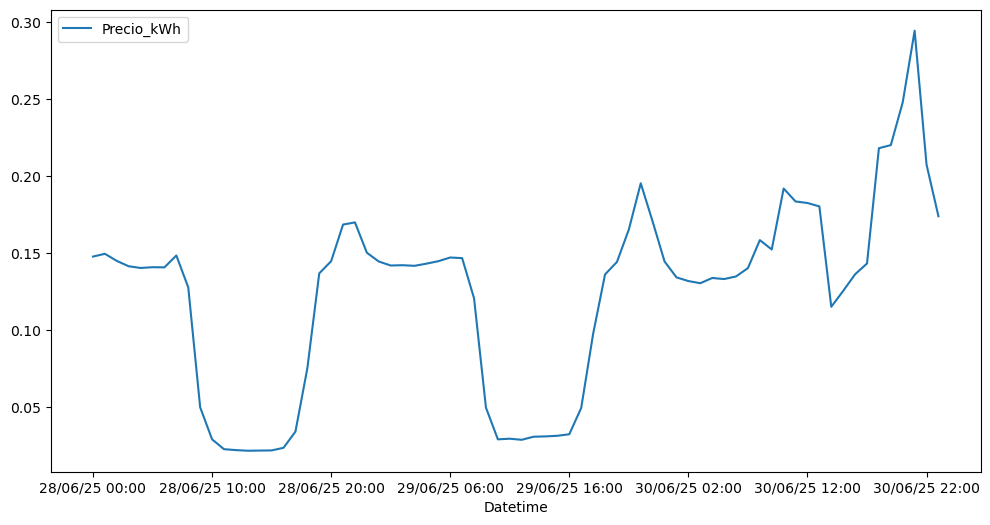
\includegraphics[width=0.6\linewidth]{figuras/histoico.png}
    \caption{Serie temporal del precio horario de la electricidad (mercado SPOT español).}
    \label{graficacometa}
\end{figure}

\begin{figure}[H]
    \centering
    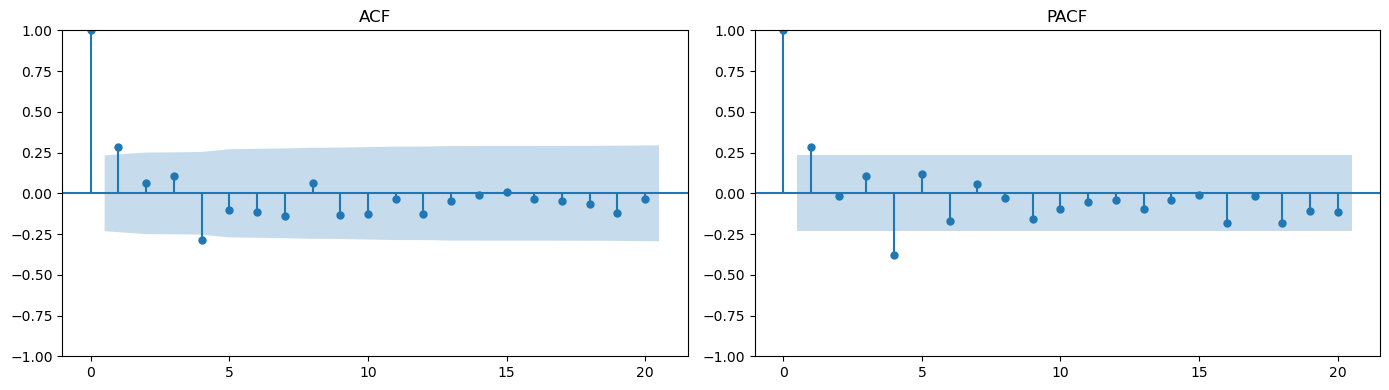
\includegraphics[width=0.6\linewidth]{figuras/ACF_PACF.png}
    \caption{Diagramas de autocorrelación (ACF) y autocorrelación parcial (PACF).}
    \label{ACFPACF}
\end{figure}

\begin{figure}[H]
    \centering
    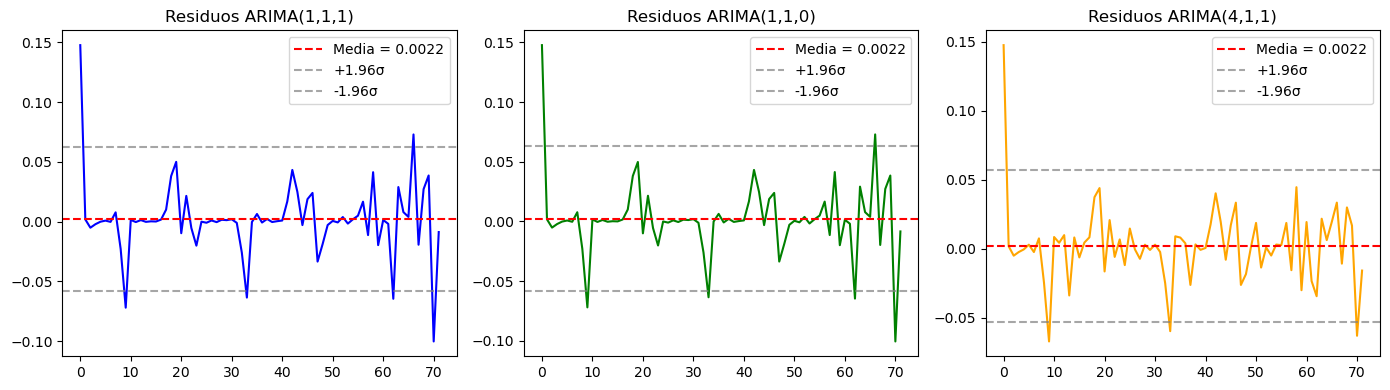
\includegraphics[width=0.6\linewidth]{figuras/residuos_ARIMA.png}
    \caption{Residuos del modelo SARIMAX tras ajuste.}
    \label{residuos}
\end{figure}

\begin{figure}[H]
    \centering
    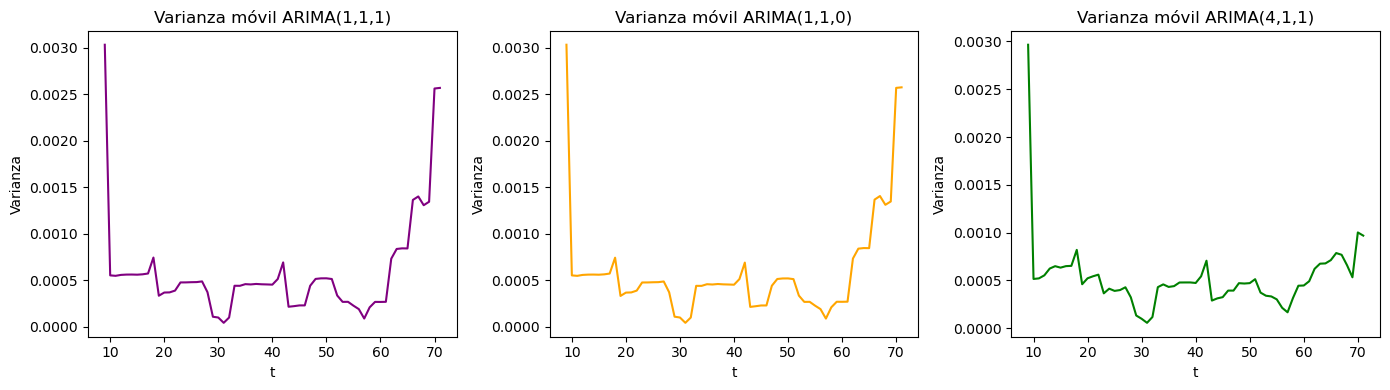
\includegraphics[width=0.6\linewidth]{figuras/varianza_ARIMA.png}
    \caption{Evaluación de la varianza residual del modelo SARIMAX.}
    \label{fig:varianaza-label}
\end{figure}

% \begin{figure}[H]
%     \centering
%     \includegraphics[width=0.6\linewidth]{figuras/TFT_predicciones.png}
%     \caption{Predicción horaria con modelo TFT (captura de código o resultados).}
%     \label{fig:tft-pred}
% \end{figure}

% \begin{figure}[H]
%     \centering
%     \includegraphics[width=0.6\linewidth]{figuras/TFT_loss.png}
%     \caption{Curva de pérdida y métricas de validación del modelo TFT.}
%     \label{fig:tft-loss}
% \end{figure}
%
%
\subsection{Modelo físico}
%
%
\subsubsection{Situación simplificada: Primera aproximación} \label{PrimeraAproximacion}
%
%
%
Dado un metal conocido (X) de temperatura de fusión $T_f$, calor específico en los estados sólido y líquido, $c_{\text{sol}}$ y $c_{\text{liq}}$ respectivamente, entonces a la hora de conocer cuánta energía será necesaria tendremos que tener en cuenta:
\begin{itemize}
    \item[I] El metal X a una temperatura inicial $T_0$ debe ser calentado hasta la temperatura de fusión $T_f$, esto dependerá del \textit{calor específico} del material en el estado \textit{sólido}, que viene a ser el \textit{coste} energético para aumentar la temperatura del mismo.
    \item[II] Una vez alcanzado dicho objetivo el material cambia de estado de la materia requiriendo una nueva cantidad de calor dependiente del \textit{calor latente} del material, denominado como $L_{\text{s-l}}$.
    \item[III] Finalmente supondremos que seguiremos elevando la temperatura por lo que, de manera análoga al paso I, tendremos que tener en cuenta esta energía. Llamaremos a este límite $T_c$
\end{itemize}
Para realizar dichos cálculos, haremos uso de las fórmulas de calor para calor específico y transiciones de fase.
\begin{align}
    Q_{\text{pf}} &= m \cdot c_{\text{sol}} \cdot (T_f-T_0).\\
    Q_{\text{f}} &= m \cdot L.\\
    Q_{\text{e}} &= m \cdot c_{\text{liq}} \cdot (T_c-T_f).
\end{align}
De este modo, $Q = Q_{\text{pf}} + Q_{\text{f}} + Q_{\text{e}}$. Finalmente, deberíamos tener en cuenta que los hornos no son ideales y tenemos una cierta pérdida de energía. Este hecho, cuantificado por el rendimiento $\eta \in [0,1]$, provoca un aumento en el calor total necesario: $Q^{\text{tot}} = Q/\eta$.

\subsubsection{Situación general} \label{SituacionGeneral}
%
%
%
Nos situamos ahora ante el problema general, en el que partimos de temperaturas iniciales cercanas a la ambiente ($T_0 \simeq 25 \C$) mientras que llegamos por lo menos a $T = 1450 \C$. En este caso tendremos que aplicar la formulación general:
\begin{equation}
    Q = m \cdot \int_{T_a}^{T_b} c(T)dT,
    \label{calor}
\end{equation}
donde $m$ es la masa del compuesto X y $c(T)$ es la función del calor específico con la temperatura. Para poder operar con esta expresión sería necesario consultar datos tabulados sobre el material y una vez obtenidos los datos de $c$ para distintas temperaturas interpolamos obtener una función con la que calcular, de manera aproximada, el calor en la \Cref{calor}.
De este modo llegaríamos a una situación similar a la descrita en la \Cref{PrimeraAproximacion}, obteniendo $Q^{\text{tot}}$. En ambos casos, como se va a tener desarrollo polinómico de $c(T)$, podemos calcular
\begin{align}
    Q & = m \cdot \int_{T_a}^{T_b} c(T)dT = m \cdot \int_{T_a}^{T_b} \Big[a_0+ a_1 T + \dots + a_nT^n \Big]dT = \\
    & = m \cdot \Big[a_0T+ \frac{a_1}{2} T^2 + \dots + \frac{a_n}{n+1} T^{n+1}\Big] \bigg|_{T_a}^{T_b} = m \cdot p(T_a, T_b),
\end{align}
donde sustituyendo obtenemos el valor deseado. Para el primer caso, tenemos que $T_a$ coincide con la temperatura \textit{ambiente} de la pieza mientras que $T_b$ con la de fusión del material X. Por otro lado, para la etapa final, la temperatura de fusión coincide con la inicial y la final, supondremos que es $1450 \C$ para todas las piezas.
\subsubsection{Traducción matemática}
La situación anterior debe ser convenientemente planteada como restricciones, de cara a la resolución del problema de optimización con el que nos encontramos. Aunando lo descrito en la \Cref{SituacionGeneral} podemos escribir que el calor $Q$ necesario para la pieza X es:
\begin{equation}
    Q = Q_{\text{pf}} + Q_{\text{f}} + Q_{\text{e}} + Q' = m \cdot \Big( p_I + L + p_{III} \Big) + Q',
\end{equation}
Donde el término $Q'$ es la energía debida a un requerimiento del fabricante, tanto de precalentamiento como de pos-fundición.\\

Finalmente, debería considerarse el rendimiento $\eta$ de los hornos. Supondremos, salvo que se indique lo contrario, que ambos hornos presentan el mismo rendimiento. Adicionalmente, dado que este valor es una constante, tenemos que $\min{\eta f(x)} = \eta \min{f(x)}$ por lo que prescindiremos de este valor puesto que no influye en la función objetivo y únicamente debería ser considerado en última instancia, a la hora de predecir el gasto estimado. Ya por último, se ha obtenido el calor $Q$ con unidad (J) \textit{julios}, mientras que habitualmente el coste eléctrico se da en \euro/kWh por lo que deberemos realizar la debida conversión. Esta, al igual que pasa con el rendimiento, influye en el valor numérico final pero no en el problema a optimizar.
%
%
\subsection{Optimización de la superficie de enfriamiento}
%
%
El presente problema aborda la distribución de las piezas metálicas recién fundidas sobre la superficie de enfriamiento disponible en la nave. Cláramente, el objetivo es maximizar el número total de piezas que pueden colocarse simultáneamente. Esta superficie cuenta además con restricciones físicas relacionadas con la seguridad y operatividad del proceso, como márgenes laterales y pasillos interiores obligatorios de al menos 1.5 metros de ancho.\\

Cada pieza fundida es clasificado según su diametro y para su manipulaciónha sido previamente colocada en una caja cuya dimensión se determina en función del tipo correspondiente. Estas cajas se disponen en planta sobre la superficie, sin posibilidad de apilarse. Una vez colocadas, las cajas no pueden solaparse ni invadir los pasillos o márgenes de seguridad. Es decir, deben respetarse las distancias mínimas entre ellas y con respecto a los bordes del área de enfriamiento. Esto impone restricciones geométricas estrictas sobre su posicionamiento.\\

El objetivo final es obtener una disposición óptima que maximice la cantidad total de piezas colocadas, permitiendo una planificación eficiente del enfriado. Dado el carácter discreto y combinatorio del problema, este puede abordarse mediante algoritmos de optimización específicos como métodos de empaquetado 2D, algoritmos genéticos o formulaciones de programación entera si se requiere una solución exacta.\\
%
%
